% Paquets généraux
\documentclass[a4paper,12pt,titlepage]{article}
\usepackage[T1]{fontenc}
\usepackage[utf8]{inputenc}
\usepackage[french]{babel}
\usepackage[gen]{eurosym}
%\usepackage[dvips]{graphicx}
\usepackage{fancyhdr}
\usepackage{pdfpages} 
\usepackage{multido}
\usepackage{hyperref}
%\usepackage{textcomp}
%\usepackage{aeguill}
\usepackage{schemabloc}
\usepackage[bitstream-charter]{mathdesign}
\usepackage{minted}

\newcommand{\id}{71}
\newcommand{\nom}{Théorie des mécanismes}
\newcommand{\sequence}{04}
\newcommand{\nomsequence}{Liaisons entre les solides}
\newcommand{\num}{02}
\newcommand{\type}{KH}
\newcommand{\descrip}{Liaisons équivalentes, hyperstatisme, liaisons en série et en parallèle, théorie des graphes}
\newcommand{\competences}{B2-12: Proposer une modélisation des liaisons avec leurs caractéristiques géométriques. \\ &  B2-13: Proposer un modèle cinématique paramétré à partir d'un système réel, d'une maquette numérique ou d'u \\ &  B2-17: Simplifier un modèle de mécanisme. \\ &  B2-18: Modifier un modèle pour le rendre isostatique. \\ &  C1-04: Proposer une démarche permettant d'obtenir une loi entrée-sortie géométrique.  \\ &  C2-05: Caractériser le mouvement d'un repère par rapport à un autre repère. \\ &  C2-06: Déterminer les relations entre les grandeurs géométriques ou cinématiques. }
\newcommand{\nbcomp}{7}
\newcommand{\systemes}{}
\newcommand{\systemesnum}{}
\newcommand{\systemessansaccent}{}
\newcommand{\ilot}{2}
\newcommand{\ilotstr}{02}
\newcommand{\dossierilot}{\detokenize{Ilot_02 }}


\newcommand{\auteurun}{Renaud Costadoat}
\newcommand{\auteurdeux}{Françoise Puig}
\newcommand{\institute}{Lycée Dorian}


\usepackage{color}
\usepackage{xcolor}
\usepackage{colortbl}
\usepackage{helvet}
\usepackage[frenchmath]{newtxsf} % for sans serif symbols
\renewcommand{\familydefault}{\sfdefault}
%\usepackage{amsfonts}
%\usepackage{amsmath}
%\usepackage{lmodern}
\usepackage{mathastext}
%\usepackage{xspace}
\usepackage{varioref}
\usepackage{tabularx}
%\usepackage{floatflt}
\usepackage{graphics}
\usepackage{wrapfig}
\usepackage{textcomp}
\usepackage{tikz}
\usepackage{wrapfig}
\usepackage{gensymb}
\usepackage[european]{circuitikz}
\usetikzlibrary{babel}
\usepackage{ifthen}
\usepackage{cancel}
\usepackage{etoolbox}
\usepackage{multirow}
%\usepackage{boxedminipage}
\definecolor{gris25}{gray}{0.75}
\definecolor{bleu}{RGB}{18,33,98}
\definecolor{bleuf}{RGB}{42,94,171}
\definecolor{bleuc}{RGB}{231,239,247}
\definecolor{rougef}{RGB}{185,18,27}
\definecolor{rougec}{RGB}{255,188,204}%255,230,231
\definecolor{vertf}{RGB}{103,126,82}
\definecolor{vertc}{RGB}{220,255,191}
\definecolor{forestgreen}{rgb}{0.13,0.54,0.13}
\definecolor{blcr}{rgb}{0.59,0.69,0.84}
\definecolor{blfr}{rgb}{0.32,0.51,0.75}
\definecolor{orfr}{rgb}{0.90,0.42,0.15}
\definecolor{orcr}{rgb}{0.90,0.65,0.50}
\definecolor{orangef}{rgb}{0.659,0.269,0.072}
\definecolor{orange}{rgb}{0.58,0.35,0.063}
\definecolor{orangec}{rgb}{0.43,0.32,0.25}
\definecolor{rcorrect}{rgb}{0.6,0,0}
\definecolor{sequence}{rgb}{0.75,0.75,0.75}
\definecolor{competences}{rgb}{0.61,0.73,0.35}
\definecolor{grisf}{HTML}{222222}
\definecolor{grisc}{HTML}{636363}
\definecolor{normal}{HTML}{4087c4}
\definecolor{info}{HTML}{5bc0de}
\definecolor{success}{RGB}{92,184,92}
\definecolor{warning}{RGB}{240,173,78}
\definecolor{danger}{RGB}{217,83,79}
\hypersetup{                    % parametrage des hyperliens
    colorlinks=true,                % colorise les liens
    breaklinks=true,                % permet les retours à la ligne pour les liens trop longs
    urlcolor= blfr,                 % couleur des hyperliens
    linkcolor= orange,                % couleur des liens internes aux documents (index, figures, tableaux, equations,...)
    citecolor= forestgreen                % couleur des liens vers les references bibliographiques
    }

% Mise en page
\pagestyle{fancy}

\setlength{\hoffset}{-18pt}

\setlength{\oddsidemargin}{0pt} 	% Marge gauche sur pages impaires
\setlength{\evensidemargin}{0pt} 	% Marge gauche sur pages paires
\setlength{\marginparwidth}{00pt} 	% Largeur de note dans la marge
\setlength{\headwidth}{481pt} 	 	% Largeur de la zone de tête (17cm)
\setlength{\textwidth}{481pt} 	 	% Largeur de la zone de texte (17cm)
\setlength{\voffset}{-18pt} 		% Bon pour DOS
\setlength{\marginparsep}{7pt}	 	% Séparation de la marge
\setlength{\topmargin}{-30pt} 		% Pas de marge en haut
\setlength{\headheight}{35pt} 		% Haut de page
\setlength{\headsep}{20pt} 		% Entre le haut de page et le texte
\setlength{\footskip}{30pt} 		% Bas de page + séparation
\setlength{\textheight}{700pt} 		% Hauteur de l'icone zone de texte (25cm)
\setlength\fboxrule{1 pt}
\renewcommand{\baselinestretch}{1}
\setcounter{tocdepth}{1}
\newcommand{\cadre}[2]
{\fbox{
  \begin{minipage}{#1\linewidth}
   \begin{center}
    #2\\
   \end{center}
  \end{minipage}
 }
}

\newcounter{num_quest} \setcounter{num_quest}{0}
\newcounter{num_rep} \setcounter{num_rep}{0}
\newcounter{num_cor} \setcounter{num_cor}{0}

\newcommand{\question}[1]{\refstepcounter{num_quest}\par
~\ \\ \parbox[t][][t]{0.15\linewidth}{\textbf{Question \arabic{num_quest}}}\parbox[t][][t]{0.93\linewidth}{#1}\par
}


\newcommand{\reponse}[1]
{\refstepcounter{num_rep}
\noindent
\rule{\linewidth}{.5pt}
\textbf{Question \arabic{num_rep}:}
\multido{\i=1+1}{#1}{~\ \\}
}

\newcommand{\cor}
{\refstepcounter{num_cor}
\noindent
\rule{\linewidth}{.5pt}
\textbf{Question \arabic{num_cor}:} \\
}

\newcommand{\titre}[1]
{\begin{center}
\cadre{0.8}{\huge #1} 
\end{center}
}


% En tête et pied de page
\fancypagestyle{normal}{%
  \fancyhf{}
\lhead{\nom}
\rhead{
\includegraphics[width=2cm]{../../img/logo}\hspace{2pt}}
\ifdef{\auteurdeux}{\lfoot{\auteurun,\auteurdeux}}{\lfoot{\auteurun}}
\cfoot{Page \thepage}}

\fancypagestyle{correction}{%
  \fancyhf{}
  \lhead{\colorbox{danger}{\begin{minipage}{0.65\paperwidth} \textcolor{white}{\textbf{Correction}} \end{minipage}} }
  \rhead{
\includegraphics[width=2cm]{../../img/logo}}
  \ifdef{\auteurdeux}{\lfoot{\auteurun,\auteurdeux}}{\lfoot{\auteurun}}
  \rfoot{\colorbox{danger}{\begin{minipage}{0.5\paperwidth} \begin{flushright}\textcolor{white}{\textbf{Correction}}\end{flushright} \end{minipage}} }}

\renewcommand{\footrulewidth}{0.4pt}

\usepackage{eso-pic}
\newcommand{\BackgroundPic}{%
\put(0,0){%
\parbox[b][\paperheight]{\paperwidth}{%
\vfill
\begin{center}
\hspace{0.5cm}\vspace{0.5cm}

\includegraphics[width=\paperwidth,height=\paperheight,%
keepaspectratio]{../../img/fond3}%
\end{center}
\vfill
}}}

\newcommand{\BackgroundPicdeux}{%
\put(25,-30){%
\parbox[b][\paperheight]{\paperwidth}{%
\vfill
\begin{center}

\includegraphics[width=\paperwidth,height=\paperheight,%
keepaspectratio]{../../img/fond4}%
\end{center}
\vfill
}}}

\begin{document}

\pagestyle{empty}

\vspace*{-3\baselineskip}

\AddToShipoutPicture*{\BackgroundPic}

\ifdef{\auteurdeux}{\begin{tabular}{>{\columncolor{gray!00}}m{.3\linewidth} m{.3\linewidth} >{\columncolor{gray!00}}m{.3\linewidth}}
Séquence : \sequence &  \multirow{3}{*}{\hspace{1cm}
\includegraphics[height=1.5cm]{../../img/logo}} &  \begin{flushright} \multirow{4}{*}{\hspace{1cm}\includegraphics[height=4cm]{img/qrcode}}\end{flushright}\\
Document : \type\num \\
 \institute \\
 \auteurun\\
 \auteurdeux
\end{tabular}}{\begin{tabular}{>{\columncolor{gray!00}}m{.3\linewidth} m{.3\linewidth} >{\columncolor{gray!00}}m{.3\linewidth}}
Séquence : \sequence &  \multirow{3}{*}{\hspace{1cm}
\includegraphics[height=1.5cm]{../../img/logo}} &  \begin{flushright} \multirow{4}{*}{\hspace{1cm}\includegraphics[height=4cm]{img/qrcode}}\end{flushright}\\
Document : \type\num \\
 \institute \\
 \auteurun
\end{tabular}}

\vspace{1cm}

\ifdef{\prive}{\begin{center}\colorbox{danger}{\Huge{Avec Correction}}\end{center}}{}

\begin{center}\huge{\nom}\end{center}

\vspace{2cm}

\ifdef{\imagedeux}{\begin{minipage}{0.49\linewidth}}{}
\begin{center}\includegraphics[height=5cm]{/home/renaud/Documents/Renaud/GitHub/django_education/systemes/\imageun}\end{center}
\ifdef{\imagedeux}{\end{minipage}\hfill
\begin{minipage}{0.49\linewidth}
\begin{center}\includegraphics[height=5cm]{/home/renaud/Documents/Renaud/GitHub/django_education/systemes/\imagedeux}\end{center}
\end{minipage}}{}

\vspace{5cm}


\begin{tabular}{p{.15\linewidth} >{\columncolor{white}}p{.8\linewidth}}
    \rowcolor{gray!20}
    Référence & S\sequence\ - \type\num \\
    Compétences & \competences \\
 	\rowcolor{gray!20}
    Description & \descrip \\
    Système & \systemes
  \end{tabular}

\newpage

\AddToShipoutPicture{\BackgroundPicdeux}

\pagestyle{normal}

\section{Définition du modèle}

Le point de départ est la représentation du corps de pompe pour ajouter les portées de noyau. 

\textbf{Etapes de Construction}

\textbf{Copier} le fichier du corps et \textbf{donner} lui le nom : MODELE. 

\textit{Supposer par la suite que les barres d'outils nécessaires ont été activées et que la case \og Saisir la Cote \fg a été cochée.}

\begin{enumerate}
 \item Création d'un bossage
 \item 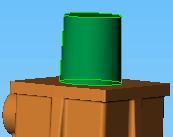
\includegraphics[height=1.5cm]{img/SW-000.png}
 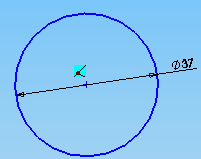
\includegraphics[height=1.5cm]{img/SW-001.png}
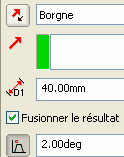
\includegraphics[height=1.5cm]{img/SW-002.png}
\end{enumerate}

En vue Perspective, \textbf{sélectionner} la face supérieure du cylindre. \textbf{Cliquer} 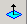
\includegraphics[height=0.4cm]{img/SW-003.png}

\textbf{Tracer} un cercle de $\Phi 37$. 
Dans la seconde barre de menus, \textbf{développer} Fonctions, puis \textbf{cliquer} Base/Bossage extrudé. 
\textbf{Entrer} la hauteur 40. \textbf{Indiquer} la valeur de l'angle de dépouille 2 \textdegree.

\begin{enumerate}
\setcounter{enumi}{2}
 \item  Création des 2 autres bossages identiques.
  \textbf{Répétez} les opérations précédentes pour les 2 autres faces supérieures des blocs-cylindre.
 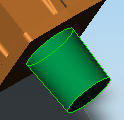
\includegraphics[height=1.5cm]{img/SW-004.png}
 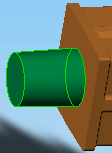
\includegraphics[height=1.5cm]{img/SW-005.png}
 \item Création d'un bossage. 
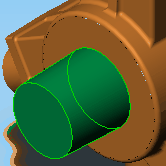
\includegraphics[height=1.5cm]{img/SW-006.png}
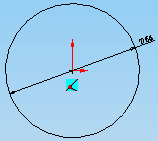
\includegraphics[height=1.5cm]{img/SW-007.png}
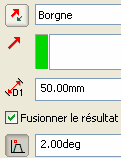
\includegraphics[height=1.5cm]{img/SW-008.png}

En vue Perspective, \textbf{sélectionner} la face latérale indiquée et \textbf{cliquer} 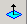
\includegraphics[height=0.4cm]{img/SW-009.png}.

\textbf{Tracer} un cercle de $\Phi 56$.
\end{enumerate}

Dans la seconde barre de menus, \textbf{développer} Fonctions, puis \textbf{cliquer} Base/Bossage extrudé. 

\textbf{Entrer} la hauteur 50. \textbf{Indiquer} la valeur de l'angle de dépouille 2\textdegree. 

\begin{enumerate}
\setcounter{enumi}{4}
 \item  Création d'un bossage
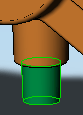
\includegraphics[height=1.5cm]{img/SW-013.png}
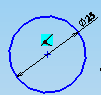
\includegraphics[height=1.5cm]{img/SW-014.png}
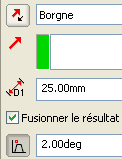
\includegraphics[height=1.5cm]{img/SW-015.png}
\end{enumerate}

En vue Perspective, \textbf{sélectionner} la face inférieure indiquée. \textbf{Cliquer} 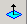
\includegraphics[height=0.4cm]{img/SW-016.png}.
  
\textbf{Tracer} un cercle de $\Phi 25$. 
Dans la seconde barre de menus, \textbf{développer} Fonctions, puis \textbf{cliquer} Base/Bossage extrudé. 
\textbf{Entrer} la hauteur 25. \textbf{Indiquer} la valeur de l'angle de dépouille 2\textdegree. 

 \begin{minipage}{0.7\linewidth}
  Il est possible de modifier la couleur en cliquant avec le bouton droit sur le nom de la pièce dans l'arborescence, puis Apparence / Couleur. 
 \end{minipage}
 \hfill
 \begin{minipage}{0.29\linewidth}
  \centering\centering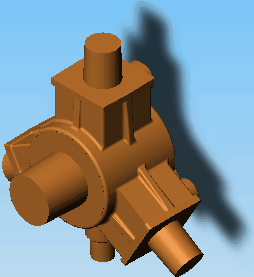
\includegraphics[height=1.5cm]{img/SW-017.png}
 \end{minipage}

\newpage

\section{Définition des noyaux}

\textbf{Créer} le noyau relatif au corps de pompe.

\textbf{Utiliser} les fonctions élémentaires de création d'un objet. 

\textbf{Etapes de Construction}

\textbf{Supposer} par la suite que les barres d'outils nécessaires ont été activées et que la case \og Saisir la Cote \fg a été cochée. 
 
\textbf{Sauvegarder} de temps en temps (nom CORPS ). 
 
\textbf{Appuyer} sur les touches \og Ctrl + N \fg , puis OK pour créer une nouvelle pièce. 

\begin{enumerate}
 \item Création d'un corps de révolution.

Dans l'arbre de création, \textbf{sélectionner} Plan de Face, puis \textbf{cliquer} 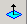
\includegraphics[height=0.4cm]{img/SW-018.png}.

\textbf{Tracez} le profil indiqué.
 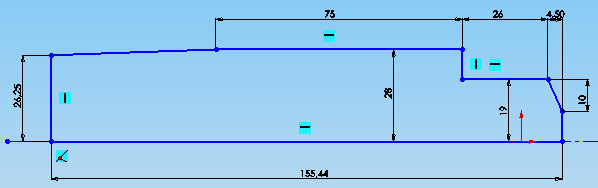
\includegraphics[height=2cm]{img/SW-019.png}
\end{enumerate}

~\

Dans la seconde barre de menus, \textbf{développer} Fonctions, puis \textbf{cliquer} Bossage/ Base avec révolution. 
\textbf{Entrer} 360° 

\begin{enumerate}
\setcounter{enumi}{1}
 \item  Création d'un bossage. 
Dans l'arbre de création, \textbf{sélectionner} Plan de Dessus, puis \textbf{cliquer} 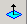
\includegraphics[height=0.4cm]{img/SW-020.png}.

\textbf{Tracer} le cercle indiqué.
 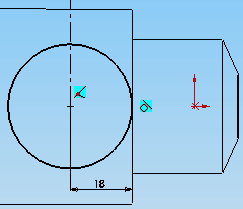
\includegraphics[height=1.5cm]{img/SW-021.png} 
 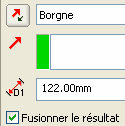
\includegraphics[height=1.5cm]{img/SW-022.png}

Dans la seconde barre de menus, \textbf{développer} Fonctions, puis \textbf{cliquer} Base/Bossage extrudé.

\textbf{Entrer} la hauteur 122. (Borgne)
\end{enumerate}

\begin{enumerate}
\setcounter{enumi}{2}
 \item  \textbf{Sélectionner} la face supérieure du cylindre nouvellement créé, puis \textbf{cliquer} 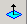
\includegraphics[height=0.4cm]{img/SW-023.png}.

\textbf{Tracer} le cercle indiqué.
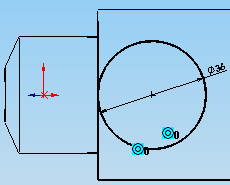
\includegraphics[height=1.5cm]{img/SW-024.png} 
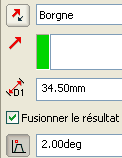
\includegraphics[height=1.5cm]{img/SW-025.png}
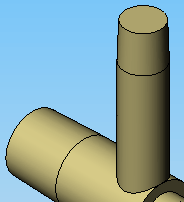
\includegraphics[height=1.5cm]{img/SW-026.png}

Dans la seconde barre de menus, \textbf{développer} Fonctions, puis  \textbf{cliquer} Base/Bossage extrudé. 

 \textbf{Entrer} les valeurs indiquées. 

 \item Création d'un bossage

Dans l'arbre de création, \textbf{sélectionner} Plan de Dessus, puis \textbf{cliquer} 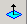
\includegraphics[height=0.4cm]{img/SW-027.png}.

\textbf{Tracer} le cercle indiqué. 
 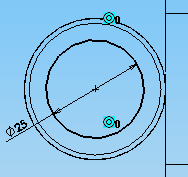
\includegraphics[height=1.5cm]{img/SW-028.png} 
\end{enumerate}

\begin{enumerate}
\setcounter{enumi}{4}
 \item  Dans la seconde barre de menus, \textbf{développer} Fonctions, puis \textbf{cliquer} Base/Bossage extrudé. 

\textbf{Entrer} la hauteur 86. (Borgne) 

\textbf{Sélectionner} la face inférieure du cylindre nouvellement créé, puis \textbf{cliquer} 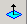
\includegraphics[height=0.4cm]{img/SW-029.png}

\textbf{Tracer} le cercle indiqué. 
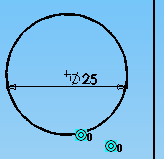
\includegraphics[height=1.5cm]{img/SW-030.png} 
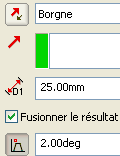
\includegraphics[height=1.5cm]{img/SW-031.png}
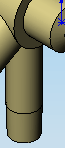
\includegraphics[height=1.5cm]{img/SW-032.png}

Dans la seconde barre de menus, \textbf{développer} Fonctions, puis  \textbf{cliquer} Base/Bossage extrudé. 

 \textbf{Entrer} les valeurs indiquées. 

\end{enumerate}


\begin{enumerate}
\setcounter{enumi}{5}
 \item   Création des 2 derniers bossages. 

Une solution revient à les créer par copie. 

Dans la seconde barre de menus, \textbf{développer} Fonctions, puis \textbf{cliquer} Répétition circulaire. 
\textbf{Se placer} en perspective pour sélectionner les éléments. 
 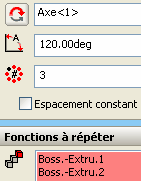
\includegraphics[height=1.5cm]{img/SW-033.png} 
\end{enumerate}

\begin{minipage}{0.7\linewidth}
Vous pouvez modifier la couleur en cliquant avec le bouton droit sur le nom de la pièce dans 
l'arborescence, puis Apparence / Couleur 
\end{minipage}
\hfill
\begin{minipage}{0.29\linewidth}
 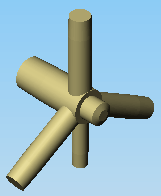
\includegraphics[height=1.5cm]{img/SW-034.png}
\end{minipage}

\newpage

\section{Définition du moule}
Z
\textbf{Créer} le moule relatif au corps de pompe. 

\textbf{Utiliser} les fonctions élémentaires de création d'un objet. 

\textbf{Etapes de Construction}

\textbf{Supposer} par la suite que les barres d'outils nécessaires ont été activées et que la case \og Saisir la Cote \fg a été cochée. 
 
\textbf{Sauvegarder} de temps en temps (nom CORPS ). 
 
\textbf{Appuyer} sur les touches \og Ctrl + N \fg , puis OK pour créer une nouvelle pièce. 

\begin{enumerate}
 \item  Création du conteneur.

Dans l'arbre de création, \textbf{sélectionner} Plan de Face, puis \textbf{cliquer} 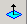
\includegraphics[height=0.4cm]{img/SW-035.png}.

\textbf{Tracez} un carré de 300x300.
\end{enumerate}

\begin{minipage}{0.29\linewidth} 
 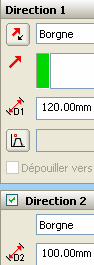
\includegraphics[width=0.5\linewidth]{img/SW-036.png}
\end{minipage}
\hfill
\begin{minipage}{0.7\linewidth}
Il faut tenir compte du modèle qui va être placé.

Le plan de face va servir de plan de joint, mais il n'est pas un plan de symétrie.

\textbf{Entrer} ce qui est indiqué. \textbf{Observer} le résultat en vue de droite par exemple.

Afin de placer correctement le modèle dans le moule, \textbf{donner} une certaine transparence au moule. 

Avec le bouton droit de la souris, \textbf{cliquer} dans l'arborescence sur Boite, puis Apparence / Couleur. \textbf{Entrer} 0,80.

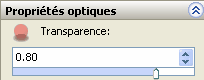
\includegraphics[height=1cm]{img/SW-037.png}
\end{minipage}
 
 ~\
 
Pour assurer la coïncidence des plans de joint lors de l'assemblage, \textbf{créer} un plan dans le plan de face.  

\textbf{Cliquer} dans la seconde barre de menus Géométrie de Référence / Plan.  

\textbf{Sélectionner} le plan de face et \textbf{indiquer} une distance 0mm (cela peut paraître redondant, mais en fait cela facilitera la sélection lors des contraintes d'assemblage). 

\textbf{Sauvegarder} le dessin : nommez le Boite par exemple.

\begin{enumerate}
 \setcounter{enumi}{1}
 \item   Création du moule. 

\textbf{Ouvrir} les dessins Corpsmodele et Boite. \textbf{Les réduire} en cliquant sur l'icône de réduction en haut de chaque fenêtre.  

\textbf{Appuyer} sur les touches \og Ctrl + N \fg, puis OK pour créer un assemblage temporaire. 

\textbf{Insérer} d'abord la Boite, puis CorpsModele en cliquant dans la seconde barre de menus sur \og Insérer des Composants \fg.

\textbf{Placer} nettement CorpsModele en dehors de la Boite. 

Il faut maintenant positionner le modèle dans le moule en indiquant la coïncidence des plans respectifs.

Dans la seconde barre de menus, \textbf{cliquer} Contraintes. Dans l'arborescence, \textbf{sélectionner} les Plan1 de Boite et de Corpsmodele. 
(On assurera ainsi la coïncidence des plans de joint)

\begin{minipage}{0.59\linewidth}
 \textbf{Se placer} en vue de face, \textbf{déplacer} ensuite Corpsmodele dans Boite. 
 (On ne peut pas déplacer le premier objet inséré qui sert de référence) 
\end{minipage}
\hfill
\begin{minipage}{0.4\linewidth}
 \centering\centering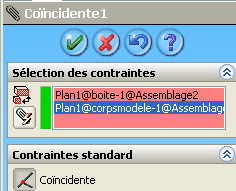
\includegraphics[height=1.5cm]{img/SW-038.png} 
\end{minipage} 
\end{enumerate}

\begin{enumerate}
 \setcounter{enumi}{2}
 \item Dans l'arborescence, avec le bouton droit, \textbf{cliquer} Boite, puis \textbf{Editer} la pièce. 

Dans la barre de menus, \textbf{cliquer} Insertion / Fonctions / Empreinte 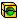
\includegraphics[height=0.4cm]{img/SW-039.png} ou Insertion / Moules / Empreinte. 

\begin{minipage}{0.6\linewidth}
 \textbf{Sélectionner} Corpsmodele dans l'arborescence et \textbf{indiquer} un facteur de retrait de 2\%. 
(En fait, celà dépend du matériau utilisé) 
\end{minipage}
\hfill
\begin{minipage}{0.39\linewidth}
 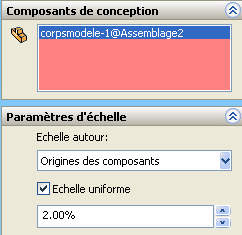
\includegraphics[height=1.5cm]{img/SW-040.png}  
\end{minipage}

 \item Création des demi-moules. 

\begin{minipage}{0.6\linewidth}
 \textbf{Sélectionner} plan1,  \textbf{cliquer} Couper la pièce. 
 
 Dans la barre de menus, \textbf{cliquer} Insertion / Moules / Fractionner 
\includegraphics[height=0.4cm]{img/SW-041.png}.
\end{minipage}
\hfill
\begin{minipage}{0.39\linewidth}
 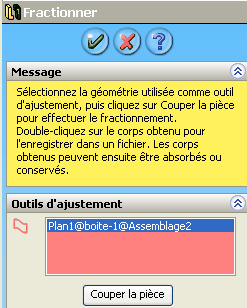
\includegraphics[height=1.5cm]{img/SW-042.png}
\end{minipage}
\end{enumerate}

\begin{enumerate}
 \setcounter{enumi}{4}
 
\item Enregistrer les pièces

\begin{minipage}{0.7\linewidth}
  Il faut maintenant enregistrer les pièces obtenues, \textbf{cocher} les cases indiquées.
 
 Renommer les moules \og mouleINF \fg  et \og mouleSUP \fg. 
\end{minipage}
\hfill
\begin{minipage}{0.29\linewidth}
 \includegraphics[height=1.5cm]{img/SW-043.png}
\end{minipage}

 \item Assemblage final. 

\begin{minipage}{0.64\linewidth}
Le travail va consister maintenant à créer un nouvel assemblage dans lequel il faudra placer, dans l'ordre : 
\begin{itemize}
 \item le moule inférieur,
 \item le noyau,
 \item le moule supérieur. 
\end{itemize}

Il est évident qu'une réalisation complète nécessite de prévoir le chemin de coulée, les évents, les masselottes d'alimentation. 
\end{minipage}
\hfill
\begin{minipage}{0.35\linewidth}
 \includegraphics[width=0.8\linewidth]{img/SW-044.png}
\end{minipage}
\end{enumerate}


\end{document}
